\chapter{実験}
本章では,人工データ実験を通して提案アプローチの性質調査と実データ解析の結果を述べる.

\section{人工データ実験}
\subsection{シミュレーション}
ニューロン集団のカルシウムイメージングデータをシミュレーションによって作り,解析手法を評価する.
シミュレーションでは1)ニューロンのネットワーク構造を作成し,2)スパイクのシミュレーションを行い,3)蛍光強度の観測データに変換する.
\subsubsection{ネットワーク構造}
シミュレーションに用いるニューロンの個数を$I$として,ニューロンのネットワーク構造を$S \in \{0, 1\}^{I \times I}$とする.
$s_{ij}$はニューロン$i$からニューロン$j$へ活動電位が伝わるかを表している.
本節では$S$の作り方を説明する.

ニューロンのネットワーク構造にはsmall world network\cite{Watts1998}を用いる.
Small world networkはノード数,張り替え確率,初期次数を決めることによってネットワークを作成するアルゴリズムである.
初期次数は,ニューロンが平均何個のニューロンとシナプス結合を持つかという変数である.
張り替え確率は,初期次数によって作成された規則的なグラフのエッジをランダムに張り替える確率である.
そのため,エッジのうち何割が遠くのニューロンとつながっているかを表す変数である.

実際のニューロンをsmall world networkによって表すために,初期次数と張り替え確率を実データから決める.
今回はこの値はニューロンのコネクションの割合と相互のコネクションの割合から決める.
興奮性ニューロン同士の6.7\%であり,そのうち双方向のコネクションの割合は24\%である\cite{Jouhanneau2015}.
発達中マウスの興奮性ニューロンから抑制性ニューロンへのコネクティビティと抑制性ニューロンから興奮性ニューロンへのコネクティビティはどちらも78\%であった\cite{Holmgren2003}.
成熟したマウスではより少ないと思われるが,データが見つからなかったため,40\%とした.
相互のコネクションの割合がランダムにエッジを作るよりも高いのは,近いニューロンにコネクションが作られやすいからだと考えられる.
これらのデータを実現するように初期次数と張り替え確率を調整した.
用いたパラメータを\Tabref{tab:parameter1}に示す.
抑制性ニューロン同士のコネクティビティは分からないため,興奮性ニューロンと同じにしている.

\begin{table}[htb]
  \center
  \begin{tabular}{|c|cc|} \hline
    結合の種類 & 初期次数 & 張り替え確率 \\ \hline
		同種類のニューロン間 & $0.0335 N$ & $0.3$ \\
		興奮性ニューロンと抑制性ニューロン間 & $0.2I$ & $0.3$\\ \hline
  \end{tabular}
  \caption{ネットワーク構造のパラメータ値}
  \label{tab:parameter1}
\end{table}

実際のネットワーク構造の作り方を説明する.
ネットワーク構造は興奮性ニューロン同士の結合,抑制性ニューロン同士の結合,興奮性ニューロンと抑制性ニューロン間の結合の3つに分けて作成する.
まず,全ニューロンのうち抑制性ニューロンと興奮性ニューロンのインデックスを決めておく.
全てのニューロンについて\Tabref{tab:parameter1}に従ってネットワークを作成し,それぞれに対応する隣接行列の上三角または下三角行列を取り出して結合する.
作成したいのは向きのある有向グラフなので,上三角行列と下三角行列を分けて作成する.

\subsubsection{スパイクシミュレーション}
スパイクのシミュレーションにIzhikevichモデル~\cite{Izhikevich2003}を用いる.
このモデルはHodgikin-Huxleyモデルをもとにしており,計算コストが低い.
Izhikevichモデルでは,あるニューロンの膜電位が閾値を超えると発火したとみなし,あらかじめ定義したニューロンのネットワーク構造に従って結合を持つニューロンの膜電位を上昇させる.
このシミュレーションで設定しなければいけないのは,個々のニューロンの特徴パラメータ,重み付きのネットワーク構造,外部からのランダムな入力である.

まず,個々のニューロンの特徴パラメータについて説明する.
このモデルではニューロンごとに4つのパラメータを設定する必要があり,そのパラメータでニューロンを特徴づける.
本論文では興奮性ニューロンにはregular spiking neurons,抑制性ニューロンにはfast spiking neuronsを用いる.
それらのパラメータを~\Tabref{tab:parameter2}に示す.
ただし,$r_e$と$r_i$は0から1の一様分布に従う確率変数である.

\begin{table}[htb]
  \center
  \begin{tabular}{|c|cccc|} \hline
    ニューロンの種類 & a & b & c & d \\ \hline
    興奮性ニューロン & 0.02 & 0.2 & $-65 + 15 r_e^2$ & $8 - 6r_e^2$ \\
    抑制性ニューロン & $0.02 + 0.08r_i$ & $0.25 - 0.05 r_i$ & -65 & 2 \\ \hline
  \end{tabular}
  \caption{Izhikevichモデルのパラメータ値}
  \label{tab:parameter2}
\end{table}

次に,重み付きのネットワーク構造$W \in \mathbb{R}^{I \times I}$について説明する.
ニューロン$i$から$j$へ結合があった場合,$w_{ij}$はニューロン$i$が発火した時にニューロン$j$の膜電位をどれだけ上昇させるかという数値である.
$W$は,前節で作成した$S$の非ゼロ要素を数値で置き換えることで作成する.
その際,同じグループへの興奮性ニューロンからの入力は強めにする.
同じグループの興奮性ニューロンからの結合は一様分布$U(7,10)$,異なるグループの興奮性ニューロンからの結合は標準偏差$\sigma_w = 1.5$の対数正規分布の$7$以下の分布,抑制性ニューロンからの結合は一様分布$U(-10,0)$からサンプルする.
対数正規分布を用いる理由は\cite{Song}のデータに基づく.
\begin{align}
	w_{ij} = \begin{cases}
		U(7,10) & (s_{ij} = 1 \text{,$i$は興奮性ニューロン,$i$と$j$は同じグループ}) \\
		\{\frac{1}{\sqrt{2 \pi \sigma_w^2}w} \exp \{ - \frac{(\ln w)^2}{2 \sigma_w^2} | w \in [0,7]\} & (s_{ij} = 1 \text{,$i$は興奮性ニューロン,$i$と$j$は異なるグループ}) \\
		U(-10,0) & (s_{ij} = 1 \text{$i$は抑制性ニューロン}) \\
		0 & (s_{ij} = 0)
  \end{cases}
	\label{eq:W}
\end{align}

最後に外部からのランダムな入力について説明する.
ニューロンには観測範囲外からの入力がある(以降,外部入力とする).
そのため,シミュレーション中も外部からの電位を乱数としてニューロンの電位に足す.
本論文では,ニューロンの活動も外部入力の大きさで表現する.
活動していない興奮性ニューロンと抑制性ニューロンにはそれぞれ,$\mathcal{N}(0,9)$と$\mathcal{N}(0,0.01)$に従う乱数を足す.
活動している興奮性ニューロンと抑制性ニューロンにはそれぞれ,$\mathcal{N}(0.5, 9)$と$\mathcal{N}(0.2,0.01)$に従う乱数を足す.
これらを\Tabref{tab:parameter3}に示す.
活動していないニューロンへの外部入力は\cite{Izhikevich2003}で用いられていたものを採用した.
ただし,興奮性ニューロンの活動時の外部入力は変化させた実験もある.

\begin{table}[htb]
  \center
  \begin{tabular}{|c|cc|} \hline
    ニューロンの種類 & 活動時の外部入力 & 活動していない時の外部入力 \\ \hline
		興奮性ニューロン & $\mathcal{N}(0.5,9)$ & $\mathcal{N}(0, 9)$ \\
		抑制性ニューロン & $\mathcal{N}(0.2, 0.01)$ & $\mathcal{N}(0, 0.01)$ \\ \hline
  \end{tabular}
  \caption{シミュレーションに用いる外部入力の値}
  \label{tab:parameter3}
\end{table}

本論文では同時に活動するニューロンを推定するのが目的の1つである.
ある時間帯にあるニューロングループが活動する時,そのニューロングループには平均値を上げた外部入力を足し,それ以外のニューロンには平均$0$の外部入力を足す.
こうすることで,ニューロングループの活動のみ上がる(つまり蛍光強度が上がる).
実際の脳でもこのように外部からの入力によってニューロンの活動を制御していると考えられる.
あるニューロングループを活動させる別の方法として,そのグループのハブとなるニューロンにのみ強い外部入力を与える方法も考えられる.

実際にマウスのニューロンの発火頻度がどれくらいなのか\cite{Watson2016}を元に\Tabref{tab:spike-frequency}に示す.
\begin{table}[htb]
  \center
  \begin{tabular}{|c|ccc|} \hline
    ニューロンの種類 & 覚醒時(Hz) & ノンレム睡眠時(Hz) & レム睡眠時(Hz) \\ \hline
		興奮性ニューロン & $0.76 \pm 1.53$ & $0.69 \pm 0.86$ & $0.88 \pm 1.33$ \\
		抑制性ニューロン & $5.59 \pm 7.25$ & $4.69 \pm 5.62$ & $4.25 \pm 9.43$ \\ \hline
  \end{tabular}
  \caption{ニューロンごとの発火頻度の中央値}
  \label{tab:spike-frequency}
\end{table}

\subsubsection{カルシウムイメージングモデル}
スパイクデータからカルシウムイオン濃度を計算する~\cite{Vogelstein2009}のモデルを用いる:
\begin{equation}
  [\text{Ca}^{2+}]_{i,t} - [\text{Ca}^{2+}]_{i,t-1} = - \frac{\Delta}{\tau}([\text{Ca}^{2+}]_{i,t-1} - [\text{Ca}^{2+}]_b) + An_{i,t} + \sigma_c \sqrt{\Delta} \epsilon_{i,t},
  \label{eq:calcium}
\end{equation}
ただし,$[\text{Ca}^{2+}]_{i,t}$をニューロン$i$の時刻$t$でのカルシウムイオン濃度,$[\text{Ca}^{2+}]_b$をカルシウムイオン濃度のベースライン,$\Delta$を時間幅,$\tau$は時定数,$A$は1つのスパイクでのカルシウムイオン濃度の上がり幅,$n_{i,t} \in \{0,1\}$はニューロン$i$の時刻$t$でのスパイク,$\sigma_c$はノイズの分散,$\epsilon_{i,t}$は標準正規分布に従う確率変数である.
この人工データでは,蛍光強度がある値から上昇しない飽和状態は考えないこととする.

次に,同論文のモデルを使ってカルシウムイオン濃度$[\text{Ca}^{2+}]_{i,t}$をカルシウムイメージングで計測される蛍光強度$F_{i,t}$に変換する:
\begin{equation}
	F_{i,t} = \alpha[\text{Ca}^{2+}]_{i,t} + \beta + \sigma_F \epsilon_{i,t},
  \label{eq:intensity}
\end{equation}
$\alpha$は強度,$\beta$はバイアス,$\sigma_F$はノイズの分散である.
\Tabref{tab:parameter2}に使用したパラメータを示す.
何種類かの蛍光タンパク質の性能を調べた論文に\cite{Chen2013a}がある.
この論文の,1秒間に10回発火した時のdecay time(蛍光強度が上がり切ってから半分の強度になるまでの時刻)から$\tau = 2.3$とし,SN比から$\sigma_c = 0.5$とした.

\begin{table}[htb]
  \center
  \begin{tabular}{c|c}
		\multicolumn{2}{c}{パラメータ値} \\ \hline
		$[\text{Ca}^{2+}]_b$ & 0.1\\
		$\Delta$ & 0.001\\
		$\tau$ & 2.3\\
		$A$ & 5.0\\
		$\sigma_c$ & 0.5 \\
		$\alpha$ & 1.0\\
		$\beta$ & 10\\
		$\sigma_F$ & 1.0\\ \hline
  \end{tabular}
  \caption{カルシウムイメージングモデルでのパラメータ値}
  \label{tab:parameter2}
\end{table}

\subsubsection{観測モデル}
実データは8[Hz]でサンプリングされたデータなので,シミュレーションした蛍光強度を125[ms]ごとに足し合わせる:
\begin{equation}
  x_{i,t'} = \sum_{t=1}^{125} F_{i,t},
  \label{eq:observation}
\end{equation}
ここで,$t'$はサンプリング後の時刻を表す.

上記の方法で作成した人工データ時系列と実データをそれぞれ\Figref{fig:art}と\Figref{fig:dat}に示す.
\begin{figure}[htbp]
    \begin{minipage}{0.5\hsize}
			\begin{center}
					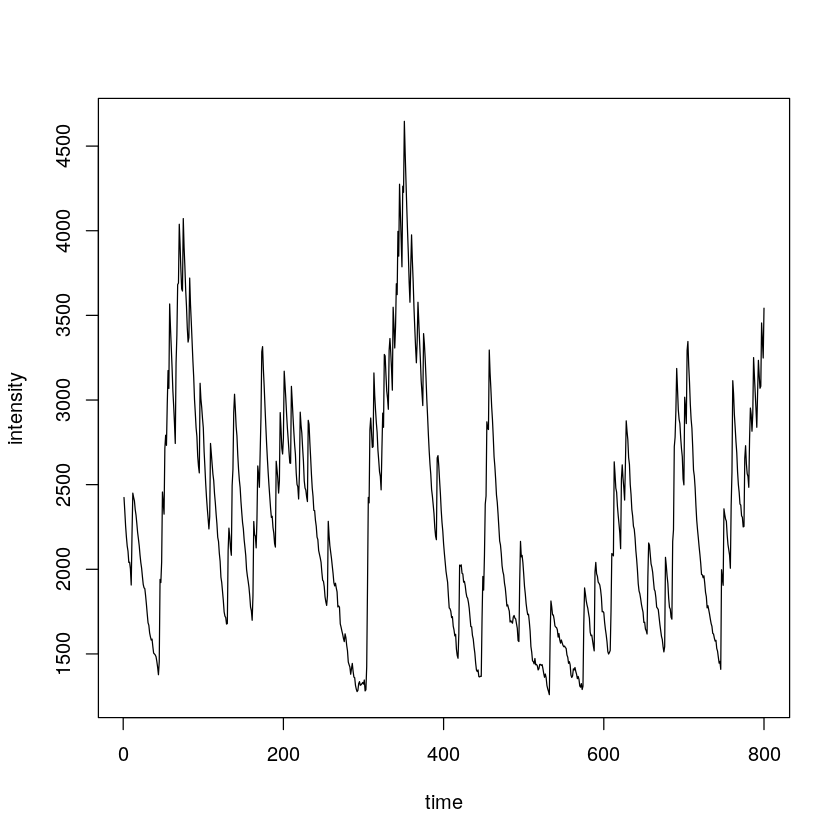
\includegraphics[width=\hsize]{artificial_data}
					\caption{人工データの時系列.}
					\label{fig:art}
			\end{center}
		\end{minipage}
    \begin{minipage}{0.5\hsize}
			\begin{center}
					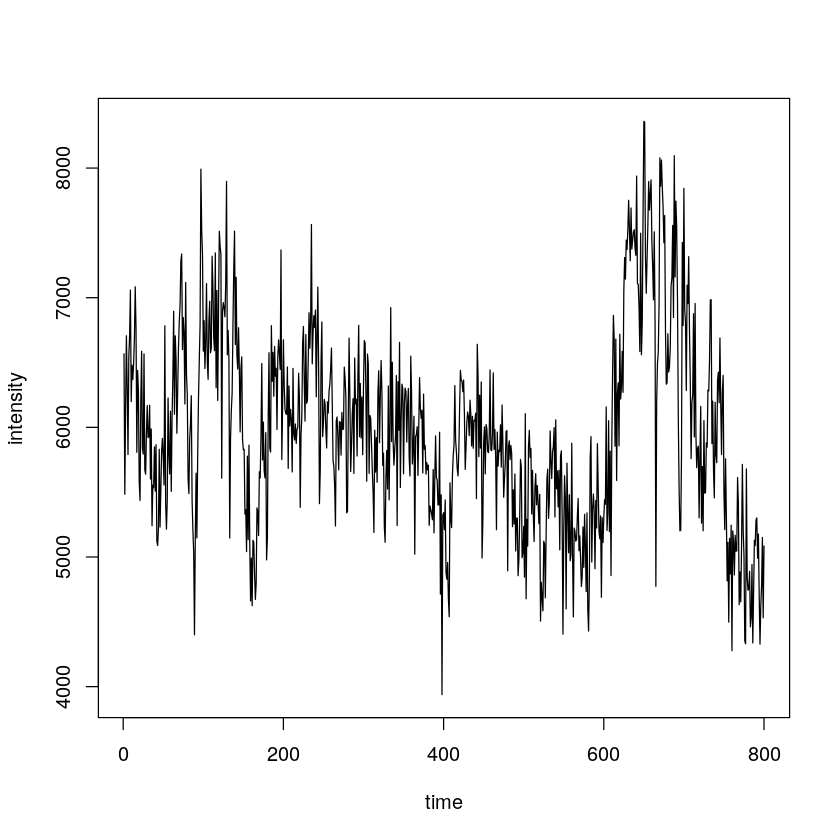
\includegraphics[width=\hsize]{real_data}
					\caption{実データの時系列.}
					\label{fig:dat}
			\end{center}
		\end{minipage}
\end{figure}

\subsubsection{実験設定}
800個の興奮性ニューロンと200個の抑制性ニューロンについてネットワーク構造$S$を作成し,\eqref{eq:W}に従って重み付きネットワーク構造$W$を作成した.
$W$は全実験を通して固定である.

$W$を元にカルシウムイメージングのシミュレーションを行った.
グループの数は10個とした.
1つのグループに所属するニューロン数は50〜200個とした.
グループが活動する時間は5[s]ごとに変えた.
ニューロングループは同時に2つまで活動することができる.
全1000個のニューロンのうち,解析に用いるのは固定された100個の興奮性ニューロンのみとする.
作成するデータの種類は以下の3種類とした.

\begin{enumerate}
  \item ニューロンは1つのグループに必ず所属する
  \item ニューロンは1つのグループに所属するかグループに所属しない
  \item ニューロンは1つか2つのグループに必ず所属し,同じニューロンが所属しているグループ同士の活動は被らない
\end{enumerate}

NMFの基底数は8から12までをそれぞれ30回ブートストラップを行った結果を用いる.
NMFの更新則はNesterov更新\cite{Guan2012}を用いる.
NMFは初期値に依存するため,本章では「NMF1回の結果」は「初期値を20回変えてNMFを行い目的関数が最小となった結果」とする.
20回は少ないかもしれないが(1000回ほどこの操作を行っている論文もある),実験サイクルを回すためにこの値にした.

\subsection{$\bar{A}$の推定に関する実験}
本節では$\bar{A}$の推定に関する結果について述べる.
実験は,5[s]ごとに1つか2つのグループが活動するデータを105[s]シミュレーションさせた結果を用いた.
ただし,最初の5[s]はシミュレーション数値の安定性のため解析から除外した.
% NMFを一回行って推定した$\hat{A}$を$\bar{A}$と比較することができるため,そのような場合はまとめて$A$と表記する.

\subsubsection{$\hat{A}(X,K)$の一意性}
前章で述べた通り,NMFには一意性がないため$\hat{A}(X,K)$にも一意性がない.
具体的には,1つの人工データについて初期値のみを変化させてNMFを行うと推定される$\hat{A}(X,K)$は同じではない.
$A$の上三角の要素について$1$と推定された頻度を調べる.
収束性と前章で述べたように寄与率が$D$の空間で取りうる値の範囲を狭めるため,$C$の行和を1とする制約を入れている.
$X$に正規化を加えなかった結果を\Figref{fig:without_scale_A}に,$X$に行和$1$の正規化を加えた結果を\Figref{fig:with_scale_A}に示す.
$X$に行和$1$の正規化を加えると,$D$の自由度は下がる.

\begin{figure}[htbp]
    \begin{minipage}{0.5\hsize}
			\begin{center}
					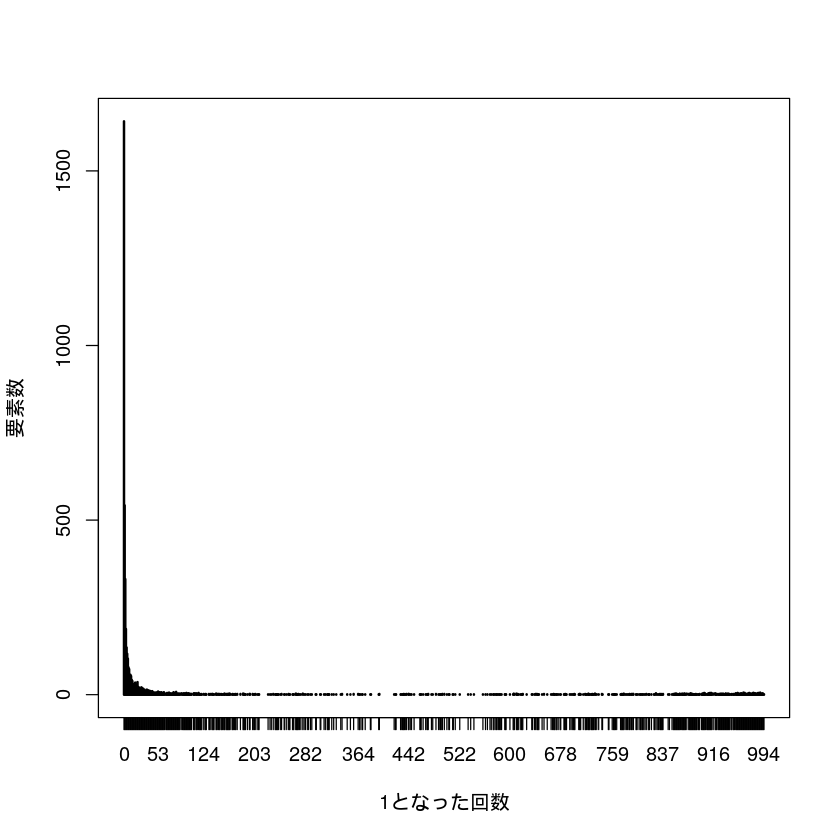
\includegraphics[width=\hsize]{without_scale_A}
					\caption{$X$を正規化せずに初期値を1000回変化させてNMFから$\hat{A}(X,K)$を推定し,各要素について$1$と推定された頻度.}
					\label{fig:without_scale_A}
			\end{center}
		\end{minipage}
    \begin{minipage}{0.5\hsize}
			\begin{center}
					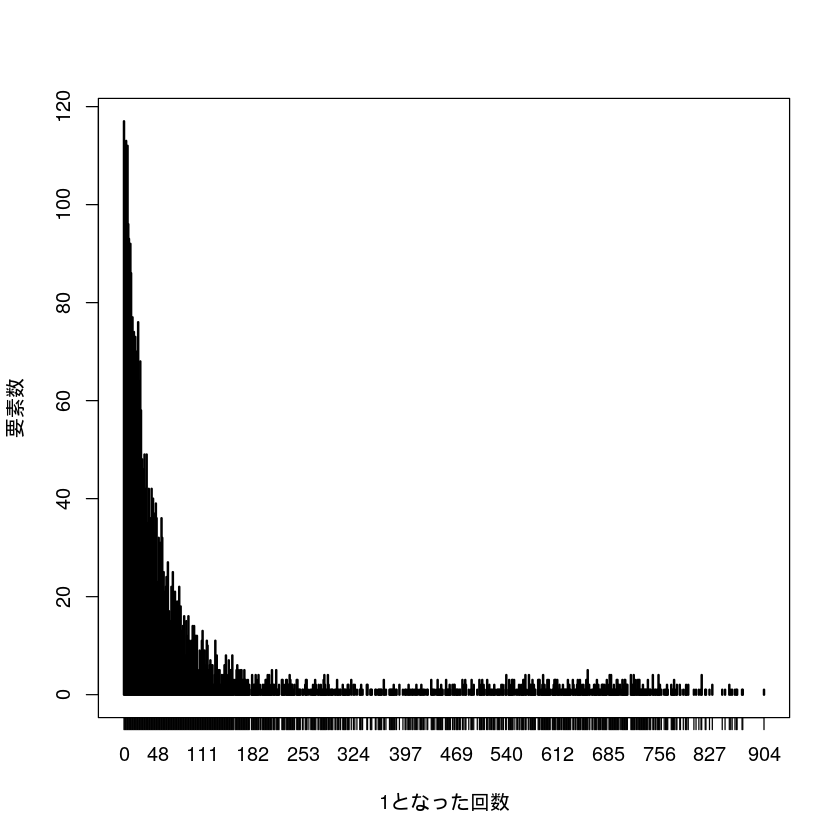
\includegraphics[width=\hsize]{with_scale_A}
					\caption{$X$を行和$1$で正規化して初期値を1000回変化させてNMFから$\hat{A}(X,K)$を推定し,各要素について$1$と推定された頻度.}
					\label{fig:with_scale_A}
			\end{center}
		\end{minipage}
\end{figure}

$\hat{A}(X,K)$に一意性がある場合は,ある$\hat{A}(X,K)$の要素が$1$と推定される回数は$0$か$1000$になる.
結果より,そうなっていないので$\hat{A}(X,K)$に一意性がないのがわかる.
また,\Figref{fig:with_scale_A}より$X$を正規化しない方がばらつきが小さい.
これは,正規化をしない方が$X$の中の大きな値に推定が引っ張られ,同じ局所解に落ちやすくなっているからだと考えられる.
また,$X$の行和1の正規化は物理的には,観測時間内のグループの活動の総和が一定であるという意味をもつ.
実際はそうではないので,今回の正規化の仕方はこの実験のみに留める.

\subsubsection{NMFの妥当性}
NMF,PCA,ICA,logistic regression,glassoの性能の比較を行った.
Logistic regressionとglassoについては筆者の卒論\cite{2018Nagayama}を参照されたい.
どちらも時間窓をスライドさせてネットワークを推定する.
今回の実験では時間窓を40,スライド幅を20とした.
Glassoのハイパーパラメータを$\rho = 0.3$とした.
一回でもエッジが張られたニューロン同士は同じグループとして推定量$\hat{A}$と同じ行列を作成した.

PCAとICAはNMFと同じく一般化線形成分分析の手法\cite{Cichocki2009}である.
PCAとICAでは$D$に相当する行列でNMFと同じように推定量$\hat{A}$を作成する.
3つの手法の基底数は10とした.

1のタイプについて100種類のデータを生成し,$\hat{A}(X,K)$を閾値$0.5$で切って$\{0,1\}^{I \times I}$の行列にした時のF1 scoreを比較した.
\begin{figure}[htbp]
    \begin{center}
        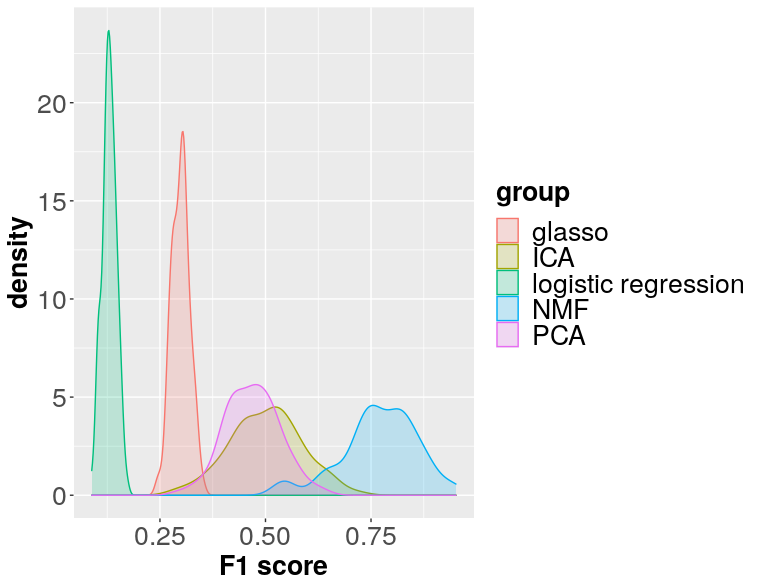
\includegraphics[width=0.5\linewidth]{compare-models}
        \caption{NMF,PCA,ICA,logistic regression,glassoのF1 scoreの密度分布}
        \label{fig:compare-models}
    \end{center}
\end{figure}
\Figref{fig:compare-models}より,NMFの精度が最も高いことが分かる.
NMFの非負制約がデータの生成モデルに合っているためだと思われる.
Glassoとlogistic regressionについては精度が低いが,各窓ごとのニューロンネットワークの活動を反映している可能性があるので,この実験のみで有用性は判断できない.

% \subsection{推定へのネットワーク構造の影響}
% グループ推定へのネットワーク構造の影響を調べるために,1と2のネットワーク構造とグループについて100種類のデータを生成し,NMFの推定精度の比較を行った.
% 人工データは,近いニューロンほどつながりやすい性質をもつので,1の人工データの方がニューロン同士が同期して活動しやすいと思われる.
% ここで,2つのニューロンが同期するとは,一方のニューロンが発火してからごく短い間にもう一方のニューロンが発火する状態が続くことである.
% 実験結果を\Figref{fig:same-exc}~\ref{fig:diff-inh}に示す.
% \begin{figure}[htbp]
%     \begin{center}
%         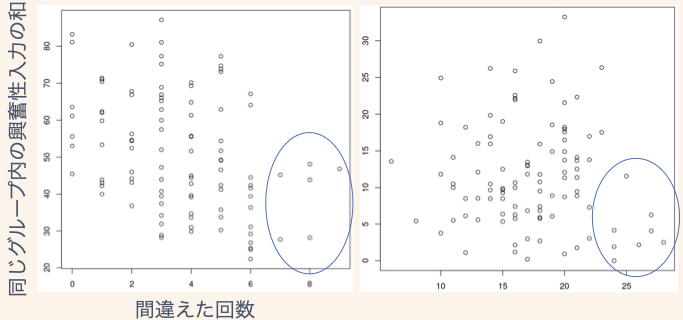
\includegraphics[width=\linewidth]{same-exc}
%         \caption{データ1と2について,ニューロンごとの間違えた回数と同じグループからの興奮性入力の和の関係}
%         \label{fig:same-exc}
%     \end{center}
% \end{figure}
% \begin{figure}[htbp]
%     \begin{center}
%       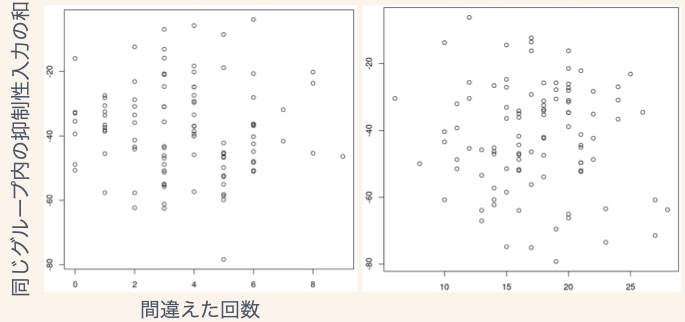
\includegraphics[width=\linewidth]{same-inh}
%         \caption{データ1と2について,ニューロンごとの間違えた回数と同じグループからの抑制性入力の和の関係}
%         \label{fig:same-inh}
%     \end{center}
% \end{figure}
% \begin{figure}[htbp]
%     \begin{center}
%         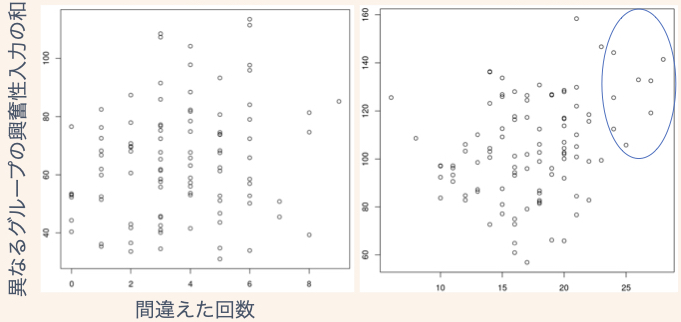
\includegraphics[width=\linewidth]{diff-exc}
%         \caption{データ1と2について,ニューロンごとの間違えた回数と異なるグループからの興奮性入力の和の関係}
%         \label{fig:diff-exc}
%     \end{center}
% \end{figure}
% \begin{figure}[htbp]
%     \begin{center}
%         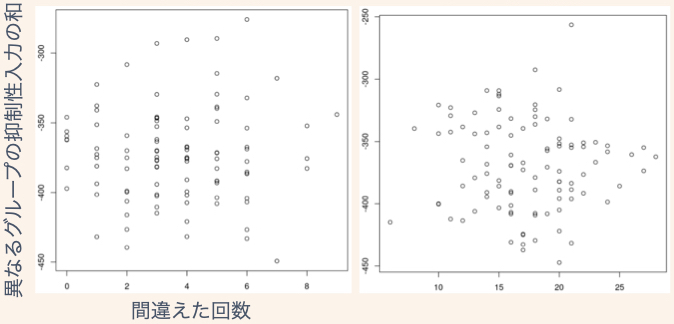
\includegraphics[width=\linewidth]{diff-inh}
%         \caption{データ1と2について,ニューロンごとの間違えた回数と異なるグループからの興奮性入力の和の関係}
%         \label{fig:diff-inh}
%     \end{center}
% \end{figure}
% \Figref{fig:same-inh},\Figref{fig:diff-inh}より,抑制性の入力は間違える回数には影響しないと思われる.
% \Figref{fig:same-exc}より,同じグループからの興奮性入力が小さいと間違えやすいと言える.
% \Figref{fig:diff-exc}より,データ2で間違える回数が多かったニューロンは異なるグループからの興奮性入力が大きかった.
% データ2ではデータ1よりも近いニューロンが異なるグループに所属する割合が多い.
% そのため,異なるグループからの興奮性入力と間違える回数の関係が強く出たと思われる.
% 
% 他にも推定へのネットワーク構造の影響の調査を試みたが,はっきりとした結果は得られなかった.

\subsubsection{ブートストラップ法とモデル平均の有用性}
ブートストラップ法で$\bar{A}(X,\mathcal{K})$を推定する有用性を確認するために,タイプ1の人工データ100個について,1回NMFを行った結果,30回初期値を変えた結果,30回ブートストラップした結果のF1 scoreを~\Figref{fig:once-init-boot}に示す.
F1 scoreの計算方法は3.2.2節と同じである.
NMFの基底数は真の基底数10を用いた.
\Figref{fig:once-init-boot}より,ブートストラップを行った方が精度が高くなることがわかる.

\begin{figure}[htbp]
    \begin{minipage}{0.5\hsize}
			\begin{center}
					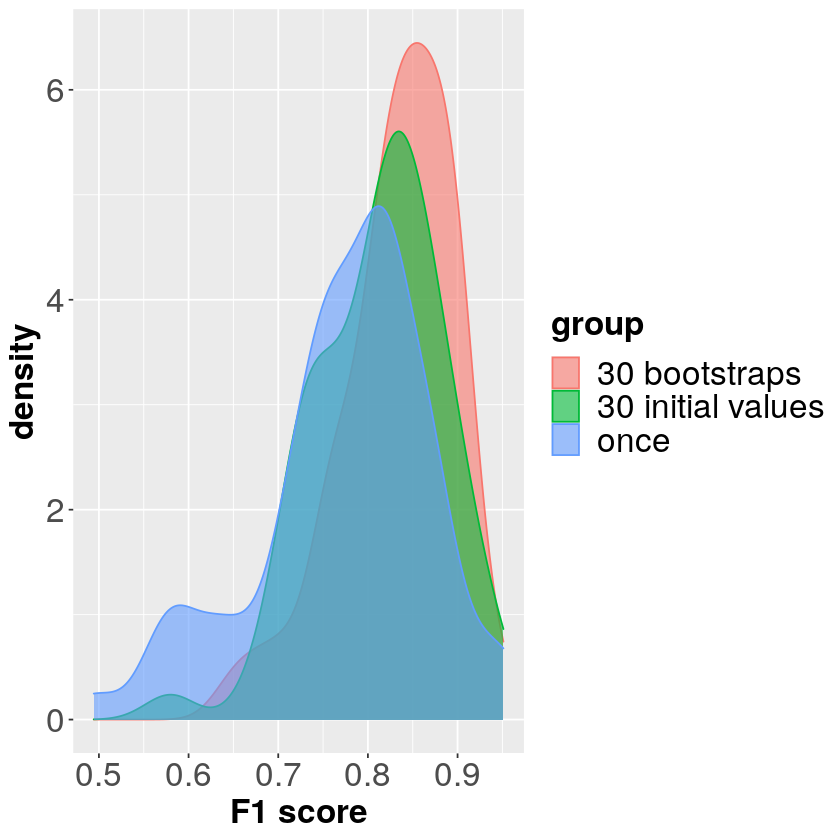
\includegraphics[width=\hsize]{once-init-boot}
					\caption{NMFを1回行った時の$\hat{A}(X,10)$,30回初期値を変えた$\hat{A}(X,10)$の平均,30回ブートストラップを行った$\bar{A}(X,\mathcal{K}); \mathcal{K} = {10}$それぞれのF1 scoreの分布.}
					\label{fig:once-init-boot}
			\end{center}
		\end{minipage}
    \begin{minipage}{0.5\hsize}
			\begin{center}
					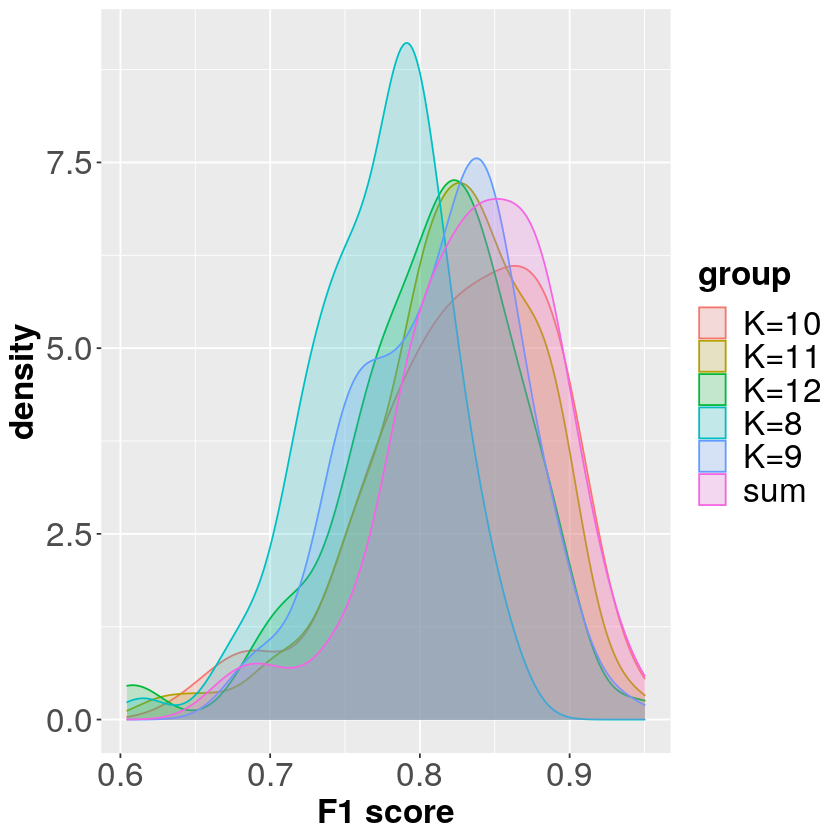
\includegraphics[width=\hsize]{f1all}
					\caption{基底数ごとにブートストラップを行った時の$\bar{A}(X,{K})$のF1 scoreと全ての基底数についてモデル平均をとった$\bar{A}(X,\mathcal{K})$のF1 scoreの分布.}
					\label{fig:f1all}
			\end{center}
		\end{minipage}
\end{figure}

基底数別に推定された$\bar{A}$とモデル平均をとった$\bar{A}$のF1 scoreを~\Figref{fig:f1all}に示す.
これより,真の基底数周りの$\bar{A}$の平均をとることである程度の精度は保たれることがわかる.

\subsubsection{NMFの基底数}
NMFの基底数を決める方法をいくつか試した.
人工データ86個についてBrunetらとUbrauらの方法で基底数を決めた時に各基底数が何回選ばれるかを~\Figref{fig:cophenetic}.\Figref{fig:uoi}に示す.
Brunetらの方法では初期値を変化させていたが,本実験ではブートストラップの結果で代用している.
Brunetらの方法では真の基底数10に近い基底数が多く選ばれているが,小さい基底数も選ばれている.
Ubaruらの方法では小さい基底数が選ばれる傾向にあった.

また,1つの人工データについてAICとAICcを計算した結果を~\Figref{fig:aic},\Figref{fig:aicc}に示す.
AICとAICcは最小となるモデルを選択する情報量基準だが,基底数が大きくなるごとに減少する傾向があった.
他の人工データについても同様の傾向にあった.

\begin{figure}[htbp]
    \begin{minipage}{0.5\hsize}
        \begin{center}
            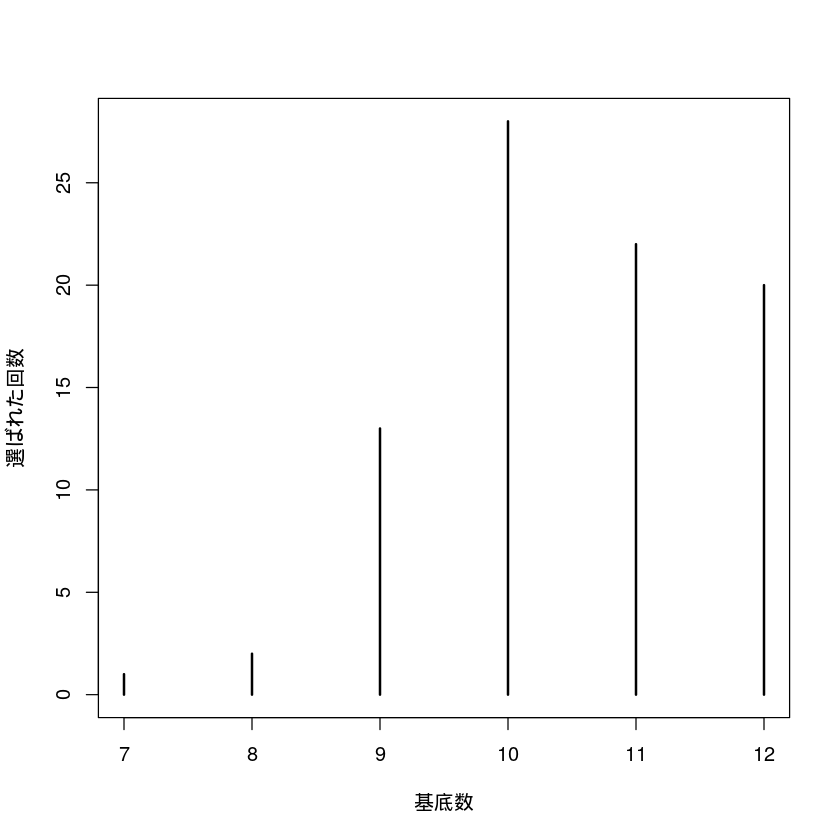
\includegraphics[width=\hsize]{cophenetic}
						\caption{Brunetらの方法で基底数を決めた時に各基底数が選ばれた回数(真の基底数は10).}
            \label{fig:cophenetic}
        \end{center}
    \end{minipage}
    \begin{minipage}{0.5\hsize}
        \begin{center}
            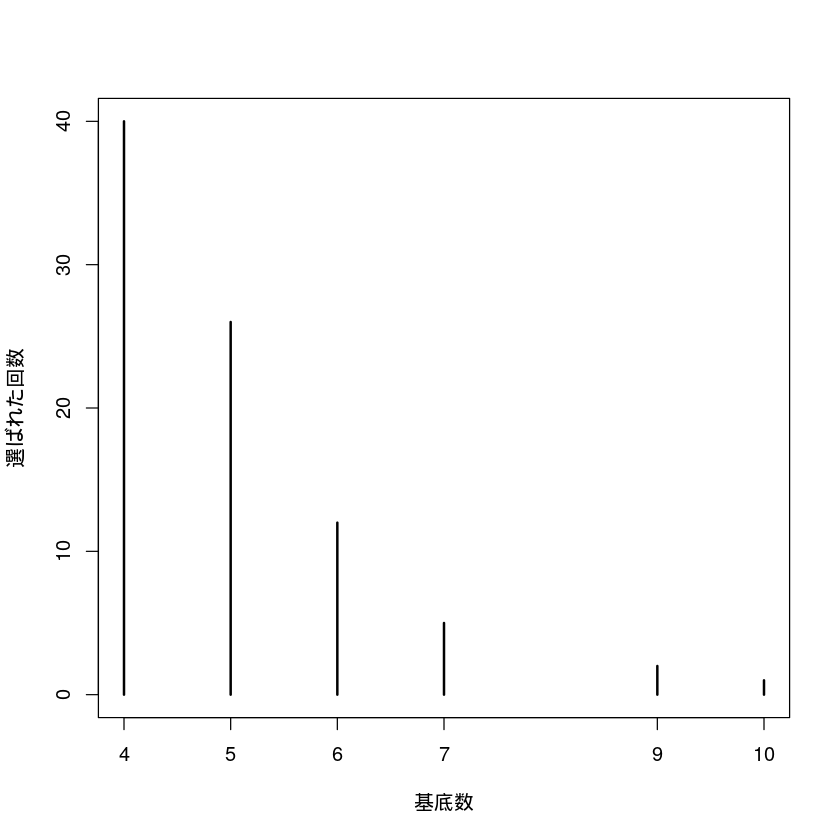
\includegraphics[width=\hsize]{uoi}
						\caption{Ubaruらの方法で基底数を決めた時に各基底数が選ばれた回数(真の基底数は10).}
            \label{fig:uoi}
        \end{center}
    \end{minipage}
\end{figure}
\begin{figure}[htbp]
    \begin{minipage}{0.5\hsize}
        \begin{center}
            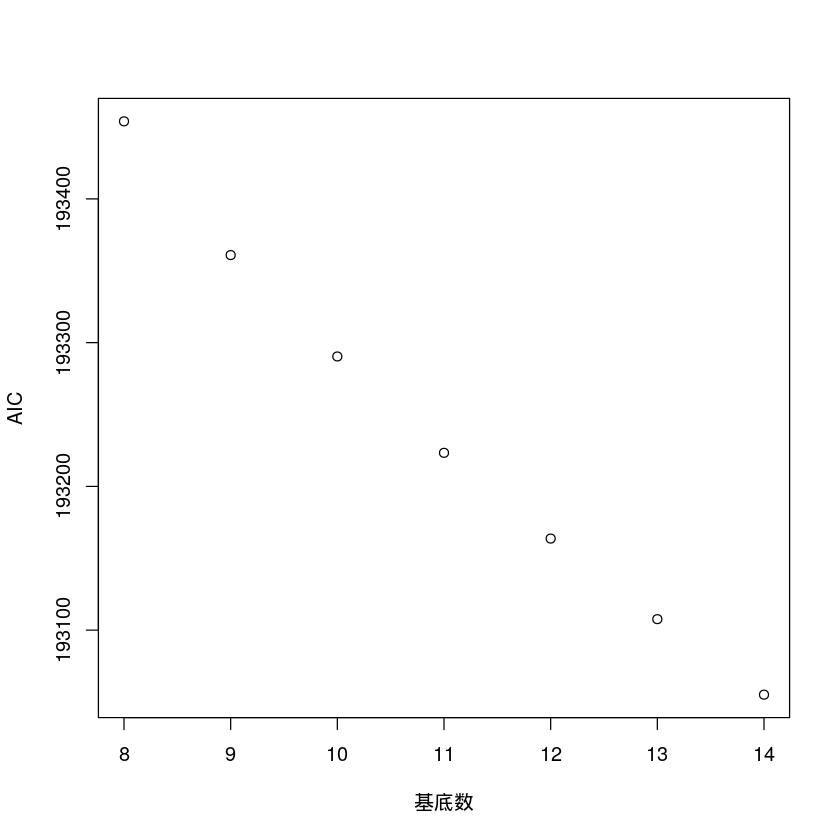
\includegraphics[width=\hsize]{aic}
						\caption{あるデータについてAICを計算した時の結果.}
            \label{fig:aic}
        \end{center}
    \end{minipage}
    \begin{minipage}{0.5\hsize}
        \begin{center}
						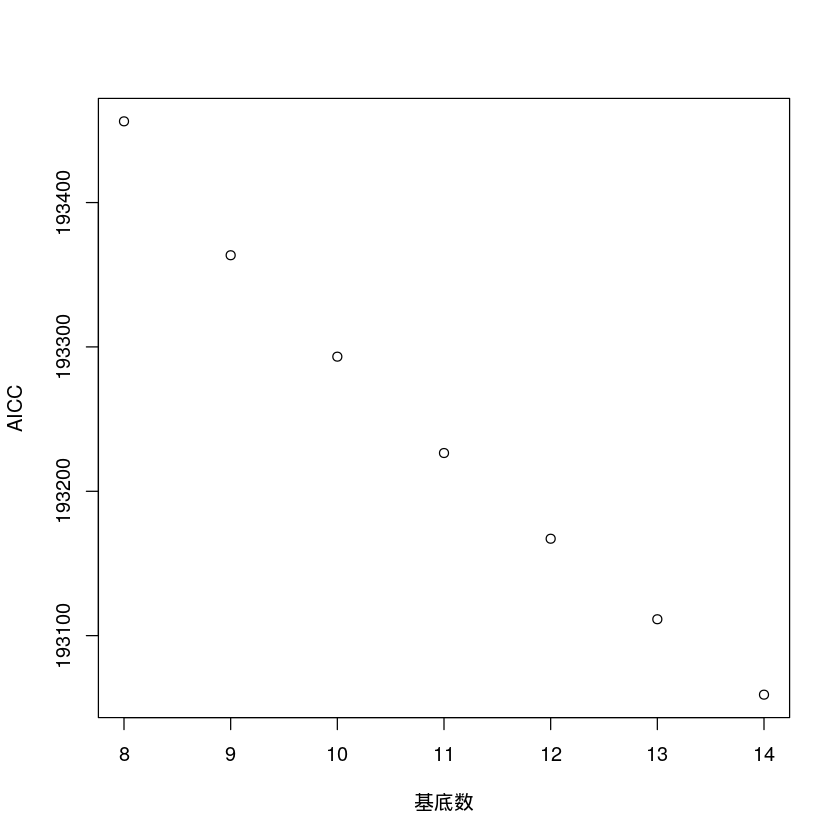
\includegraphics[width=\hsize]{aicc}
						\caption{あるデータについてAICc\cite{Symonds2011}を計算した時の結果.}
            \label{fig:aicc}
        \end{center}
    \end{minipage}
\end{figure}

\subsection{$\bar{A}$のクラスタリングに関する実験}
得られた類似度$\bar{A}$についてスペクトラルクラスタリングを行い,精度を確かめる.
比較手法には\cite{Molter2018}で性能の良かったICA-CSを用いる.
また,相関行列をk近傍法($k=20$)で$\{0,1\}$の行列にしたものとも比較を行う.
ここで注意したいのは,実データを扱う際には$k$をどう設定すればいいか分からない.
また,グループ内のニューロン数に大きな差がある場合はk近傍法ではうまく推定できないことが考えられる.
よって比較のために相関行列に易しい設定をとった.

\subsubsection{実験設定}
人工データのシミュレーション時間を実データと同じになるように905[s]とする.
ただし,最初の5[s]は安定性のため解析には用いない.
また,興奮性ニューロンに対する強い外部入力の平均を$0.5$とした.
作成した人工データの種類を\Tabref{tab:art_dat}に示す.
900[s]のシミュレーションではニューロングループは5[s]活動する機会が180回与えられる.
7200[s]のシミュレーションでは180回活動する機会がある.
all-activeは180回のうち全てでどれかのグループが活動するデータである.
non-active1は180回のうち120回活動,non-active2は60回活動するデータである.
それぞれのデータを$50$個ずつシミュレーションを行った.

NMFの設定は3.2節と同じである.
基底数は8から12までとして,それぞれ30回ブートストラップを行った結果を用いる.

\begin{table}[htb]
  \center
  \begin{tabular}{|c|c|} \hline
    人工データの種類 & 特徴 \\ \hline
		all-active & 全活動可能回数で活動 \\
		non-active1 & 活動可能回数180回のうち120回活動 \\
		non-active2 & 活動可能回数180回のうち60回活動 \\ \hline
  \end{tabular}
  \caption{人工データの種類}
  \label{tab:art_dat}
\end{table}

\subsubsection{全てのニューロンが1つのグループに所属する場合}
3種類のデータについて,$\bar{A}$と相関行列のスペクトラルクラスタリング,ICA-CSでクラスタリングを行った.
真のクラスタとのBest Match score(以降BMS)を算出した結果を\Figref{fig:bms}に示す.
\begin{figure}[htbp]
    \begin{center}
        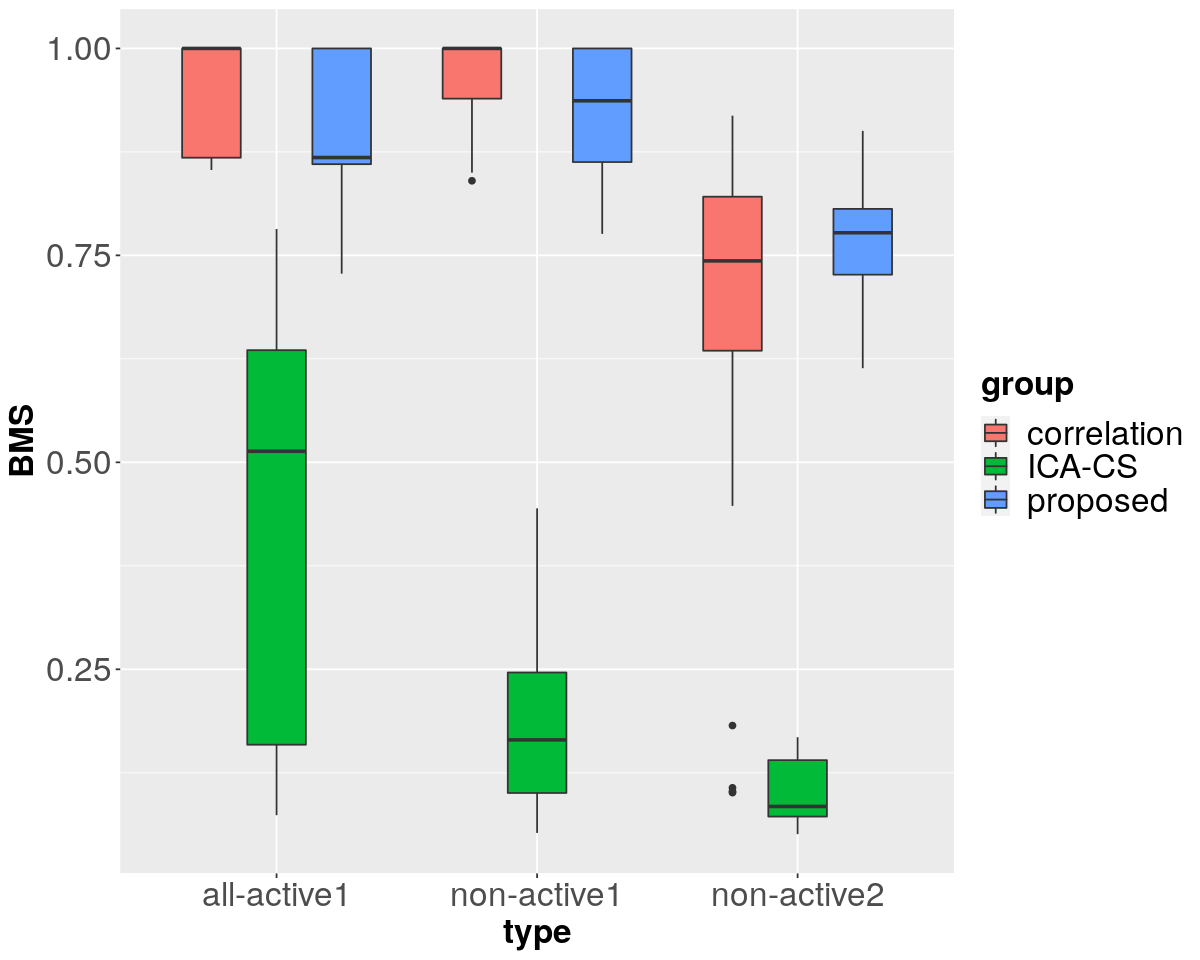
\includegraphics[width=0.8\linewidth]{bms}
        \caption{3種類の人工データについて提案手法,相関行列,ICA-CSでクラスタリングをした結果.}
        \label{fig:bms}
    \end{center}
\end{figure}
ニューロングループの活動が多い時は相関行列のBMSが最も高いが,活動しない時間が長くなると提案手法のBMSの方が良くなる.
相関行列のうち低いBMSがあるのは,クラスタ数が適切に決められなかったためだと思われる.
ICA-CSのBMSは全てのデータにおいて最も低い.
元の論文では,ICA-CSのパフォーマンスが安定して高いのはシミュレーション時間が1800[s]以上となる時だったため,データ不足が考えられる.

\subsubsection{グループに所属しないニューロンがある場合}
グループに所属しないニューロンは
